\documentclass[11pt, aspectratio = 169]{beamer}

\usetheme[progressbar=frametitle]{metropolis}
\usepackage{appendixnumberbeamer}
\usepackage{booktabs}
\usepackage[scale=2]{ccicons}
\usepackage{pgfplots}
\usepgfplotslibrary{dateplot}
\usepackage{xspace}
\usepackage{hyperref}  
\usepackage{amsmath}
\usepackage{bbm}
\usepackage[dvipsnames]{xcolor}
\usepackage{graphicx}
\usepackage{subcaption}
\usepackage{verbatim} 
\usepackage{listings}
\newcommand{\themename}{\textbf{\textsc{metropolis}}\xspace}
\definecolor{links}{HTML}{1B1B81}
\hypersetup{colorlinks,linkcolor=blue,urlcolor=blue}

% listings: To highlight code:
\usepackage{listings}
\lstset{
  language=R,
  basicstyle=\ttfamily\footnotesize,
  keywordstyle=\color{blue},
  commentstyle=\color{green!50!black},
  stringstyle=\color{red},
  frame=single,
  showstringspaces=false
}
\lstset{basicstyle=\ttfamily\footnotesize, frame=single}

\title{Applied Economics}
\subtitle{Regression Discontinuity Design}
\author{Pello Aspuru}
\date{}
\institute{Winter 2025/26}
% \titlegraphic{\hfill\includegraphics[height=1.5cm]{logo.pdf}}
\setbeamercolor{normal text}{fg=black}
\setbeamercolor{block title}{fg=teal}
\setbeamercovered{transparent} % default faintness (~15%)

\let\svdescription\description
\let\svenddescription\enddescription
\renewenvironment{description}{%
	\svdescription%
	\let\svitem\item%
	\renewcommand\item[1][]{\svitem[\textcolor{\descriptioncolor}{##1}]}%
}{
	\svenddescription%
}
\newcommand\descriptioncolor{teal}

%\usepackage{Sweave}
\begin{document}
%\Sconcordance{concordance:AE_w11_RDD.tex:AE_w11_RDD.Rtex:%
1 40 1 1 0 416 1}

	
	\maketitle
	

\begin{frame}{Introduction}
For any generic multiple linear regression model, always assume endogeneity:
\begin{align*}
       Y_{i} = \beta_0 + \beta_1 X_{1,i} + \alert{u_{i}}, \quad \quad i = 1, ... , n
	   \quad \quad E[X_{1,i} \alert{u_{i}}] \neq 0 
\end{align*}    
\pause
Four \color{teal}\textbf{quasi-experimental methods} \color{black}to \textit{mimic random treatment assignment,} overcome endogeneity, and claim \alert{causality}: 
\begin{enumerate}
    \item instrumental variables (IV) $\quad \rightarrow \quad$ Requires instrument $Z_{i}$
    \item Panel Data Methods $\quad \rightarrow \quad$ Requires Panel Data
    \item Diff-in-diff (DiD) $\quad \rightarrow \quad$ Requires Panel Data + Treatment \& Control Groups
    \item This session: \alert{Regression discontinuity design (RDD)}
\end{enumerate}

\pause

\end{frame}
	
\begin{frame}{RDD - Basic idea}

When continuous variable $a_i$ passes cutoff $c$, probability of treatment $D_{i}$ jumps to 1.
		\begin{itemize}
				\item If observation $i$ is above thresold $a_{i} > c$ $\quad \rightarrow \quad D_i =1$ gets treated.
				\item If observation $i$ is below thresold $a_{i} \leq c$ $\quad \rightarrow \quad D_i =0$ does not get treated.
				%\item[$\star$] No panel data requried.
		\end{itemize}
		\pause
		\begin{block}{Key Assumption}
			\vspace{0.2cm}
			Observations \textit{around} cutoff $c$ are \textbf{similar}, but for treatment status.
			$$
			E[u_{i} D_i] = 0
			$$
			\vspace{-1cm}
			\begin{itemize}
			\item[$\rightarrow$] \textit{As if} the treatment was randomly assigned around the cutoff! 
			\end{itemize}
		\end{block}
		\pause 
		\begin{block}{Examples of Arbitrary Cutoffs}
			\begin{itemize} \footnotesize{
				\item Treatments for "low birth weight" newborns (\textbf{$>$1,500 grams}) \footnotesize{(Almond et al., 2010)}
				%\item Legal drinking age (Carpenter and Dobkin, 2009).
				\item First-past-the-post elections (Bazzi et. al., 2025).}
			\end{itemize}
		\end{block}
\end{frame}

\begin{frame}{RDD - Pros \& Cons}
				Gap in outcome at the threshold  = $\delta$ = \textit{local} average treatment effect (LATE)
				\medskip 
		\pause
		\begin{itemize}
			\item RDD only tells you the impact of treatment on outcome \textbf{around the cutoff value} of the running variable. \color{gray}(e.g. effect of getting medical treatment at 1,500g) \color{black}
			\item	Limited \textbf{external validity}: you cannot extrapolate to the entire population. \color{gray}(e.g. effect of getting medical treatment at 3,000g birth weight) \color{black}
			\item	RDD is a very \textbf{data-hungry method}: only works with sufficiently large samples, because we essentially throw away observations that are not close to the cutoff.	
			\pause
			\item[$\rightarrow$] Does not require a panel dataset! 
		\end{itemize}
\end{frame}

\section{Example: Mortality Effect of Alcohol Consumption}

\begin{frame}[fragile]{RDD Framework - Example}
	\begin{center}
		Does alcohol consumption \alert{cause} higher mortality among young adults?
	\end{center} \pause
	Examples of endogeneity? \pause We need a random allocation of the alcohol consumption treatment
	$\rightarrow$ 	We need quasi-random variation in alcohol consumption
		\pause
		\bigskip
		\\
		In the US, alcohol consumption is prohibited before $age$ reaches the cutoff \textbf{$c=21$}.
		\medskip
		\\
		Treatment status $D_a$ is a \alert{deterministic} and \alert{discontinuous} function of $age$:
		\[
		D_a =
		\begin{cases}
		1 & \text{if } age \ge 21 \\
		0 & \text{if } age < 21
		\end{cases}
		\]
	\vspace{0.2cm}
	\pause
	\begin{lstlisting}[language=R]
	df <- read.csv("./AE_week11_RDD/dataRDD.csv")
		\end{lstlisting}
	\vspace{-0.2cm}
	\begin{itemize}
		\item[$\rightarrow$] What is the dataset's unit of observation?
	\end{itemize}
	\end{frame}

	\begin{frame}[fragile]{First Look at the Data}
	Scatterplot showcasing the three variables of interest:
	\begin{itemize}
		\item Running covariate: $age$ in years $\rightarrow$ Horizontal Axis
		\item Treatment indicator: $D_a$ $\rightarrow$ Color code
		\item Outcome variable: $Deathrate_a$ $\rightarrow$ Vertical Axis
	\end{itemize}
	\vspace{0.5cm}
	\pause
	\begin{lstlisting}[language=R]
	rdd_plot<-
	ggplot(df, aes(x = age_cell, y = death_rate_per_100T,
 			       color = as.factor(treat))) +
	geom_point(size = 2, alpha = 0.7) +
	geom_vline(xintercept = 21, linetype = "dashed") +
	theme_minimal()+theme(legend.position = "none")
		\end{lstlisting}
	\end{frame}
	
	\begin{frame}{RDD - Graphs: Running Variable and Cutoff}
		
		\begin{figure}
			\centering
			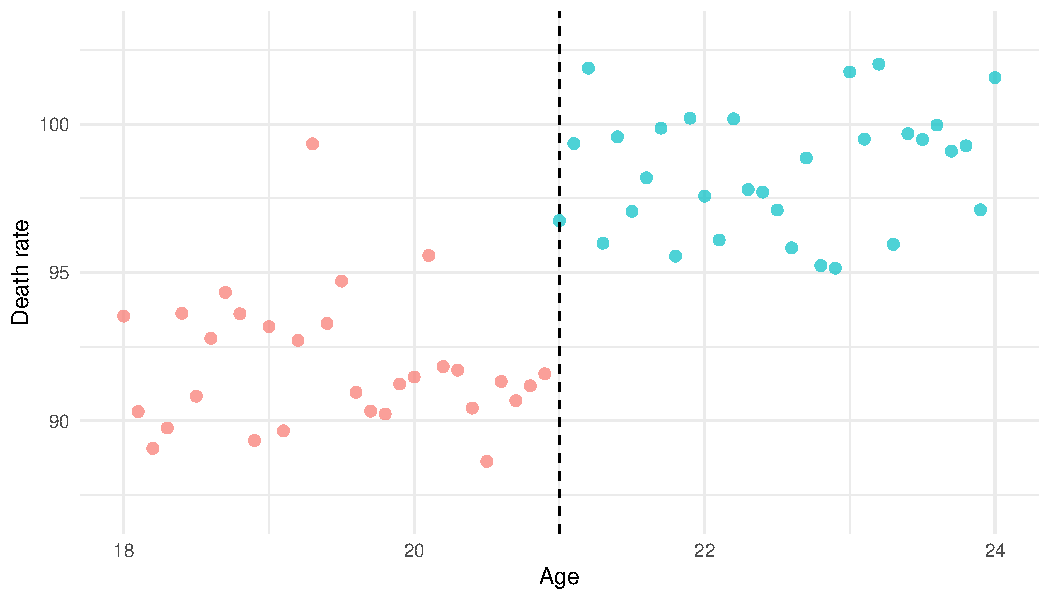
\includegraphics[width=0.83\linewidth]{RDD_graph_1.pdf}
			%\caption{Discontinuity in Treatment Status at the Cutoff}
			%\label{fig:rdd1}
		\end{figure}
	\end{frame}

\begin{frame}[fragile]{Estimation of the size of the gap}
We can write the following simple regression model: 
\begin{align*}
	Deathrate_a = \alpha + \beta (a-cutoff) + \alert{\delta}  D_a + u_a 
\end{align*}
\begin{lstlisting}[language=R]
df$age_centered <- df$age_cell - 21 # New variable centered at cutoff.
rdd_lm <- lm(death_rate_per_100T ~ age_centered + treat, data=df)
\end{lstlisting}
\begin{itemize}
		\item $Deathrate_a$ death rate at age $a$, per 100,000 people.
		\item $(a-cutoff)$ age in years, centered at the cutoff. \pause
		\item $D_a$ treatment indicator. \pause
		\item[$\rightarrow$] \alert{$\delta$} captures the ``jump'' in death rates above and below the 21 year old threshold.
\end{itemize}
\pause
RDD exploits a discontinuity at  $a = 21$ in the conditional expectation function:
\begin{align*}
	\alert{\delta} =
	\underbrace{\lim_{a \rightarrow 21^{+}} \mathbbm{E}[deathrate_a | a = c]}_{\alpha + \alert{\delta}} - \underbrace{\lim_{a \rightarrow 21^{-}} \mathbbm{E}[deathrate_a | a = c]}_{\alpha}
\end{align*}
\end{frame}

\begin{frame}[fragile]{Plotting the Regression}
	Generate the fitted values from the regression:
	\begin{lstlisting}[language=R]
	df$fit_common_slope <- predict(rdd_lm)
	\end{lstlisting}
	\pause
	Add the fit line to the previous plot:
	\begin{lstlisting}[language=R]
	geom_line(
		data = subset(df, age_cell < 21),
		aes(y = fit_common_slope, color = as.factor(treat)),
		linewidth = 1
	) +
	geom_line(
		data = subset(df, age_cell >= 21),
		aes(y = fit_common_slope, color = as.factor(treat)),
		linewidth = 1
	) +
	\end{lstlisting}
\end{frame}

\begin{frame}{Visualizing the Regression Discontinuity}
	\only<1>{
	\begin{figure}
		\centering
		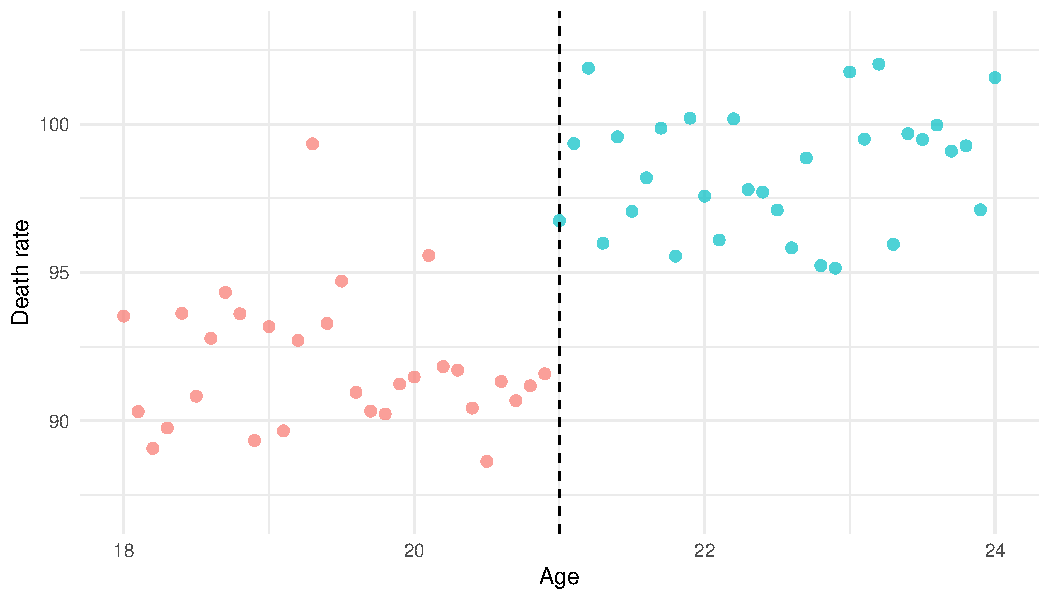
\includegraphics[width =.8\linewidth]{RDD_graph_1.pdf}
	\end{figure}}
	\only<2>{
	\begin{figure}
		\centering
		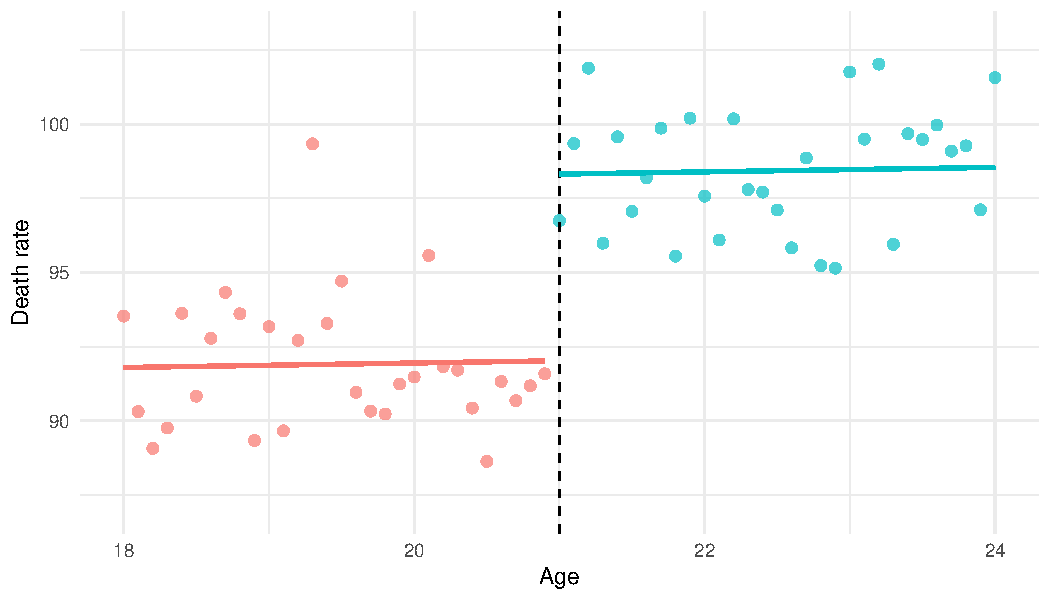
\includegraphics[width =.8\linewidth]{RDD_graph_2.pdf}
	\end{figure}}
\end{frame}

\section{Identification and Sources of Bias}

\begin{frame}{Identifying Assumption}
				\alert{Key assumption:} Potential outcomes are smooth at the threshold. In other words, in the absence of treatment, there would be no discontinuity.
				\begin{itemize}
					\item Units around the cutoff are equivalent but for treatment assignment.
					\item The only thing that changes at the cutoff must be the treatment status
					\[E[u_{i} | D_i] = 0\]
					\pause 
					\vspace{-1cm}
					\item[$\rightarrow$] Is this assumption testable?
				\end{itemize}
				\pause 
				\begin{block}{Placebo Test}
					\begin{itemize}
						\item Check if other control covariates $X_{a}$ vary at the cutoff. Which \pause
						\item If covariates are different above/beyond discontinuity... is it good or bad?
					\end{itemize}
				\end{block}				
\end{frame}

\begin{frame}{Running Covariate Manipulation}
	\vspace{-0.5cm}
	\[\text{Running Covariate } (age_i) \; + \; \text{Threshold } (age_i=21) \; \rightarrow \; \text{Treatment allocation } (D_i)\]
	\vspace{-0.5cm}
	\begin{itemize}
		\item Sometimes, units can manipulate their running covariate, decide their treatment.
		\item[$\rightarrow$] Treatment no longer randomly assigned around the cutoff! 
	\end{itemize}
\pause
Example: food labelling policies. Products with certain calories must display a warning.
\begin{overlayarea}{\textwidth}{0.55\textheight}
\only<3>{
\begin{figure}[htbp]
    \centering
    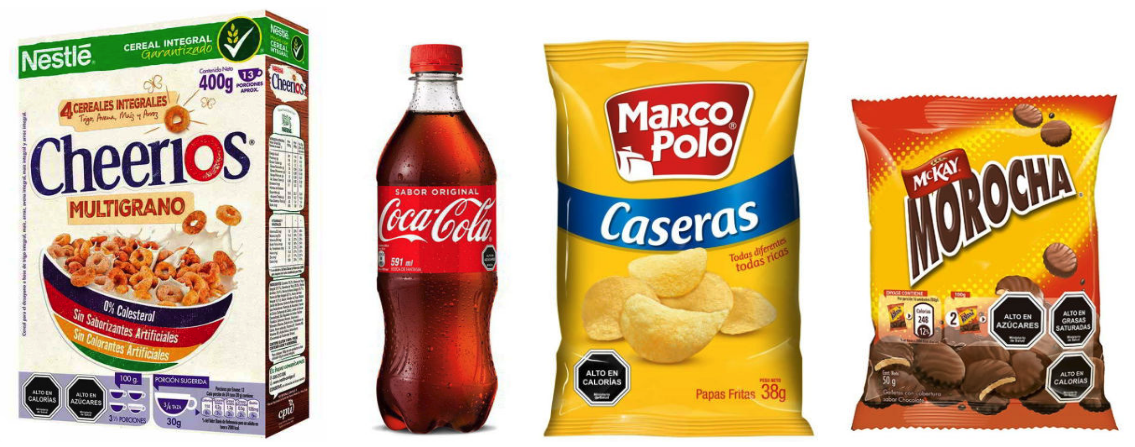
\includegraphics[trim=0cm 0cm 0cm 0cm, clip, width=0.7\linewidth]{foodlabel_2.png}
%\caption{First subfigure}
%\label{fig:sub1}
\end{figure}}
\only<4>{
\begin{figure}[htbp]
  \centering
  \begin{subfigure}[b]{0.48\textwidth}
    \centering
	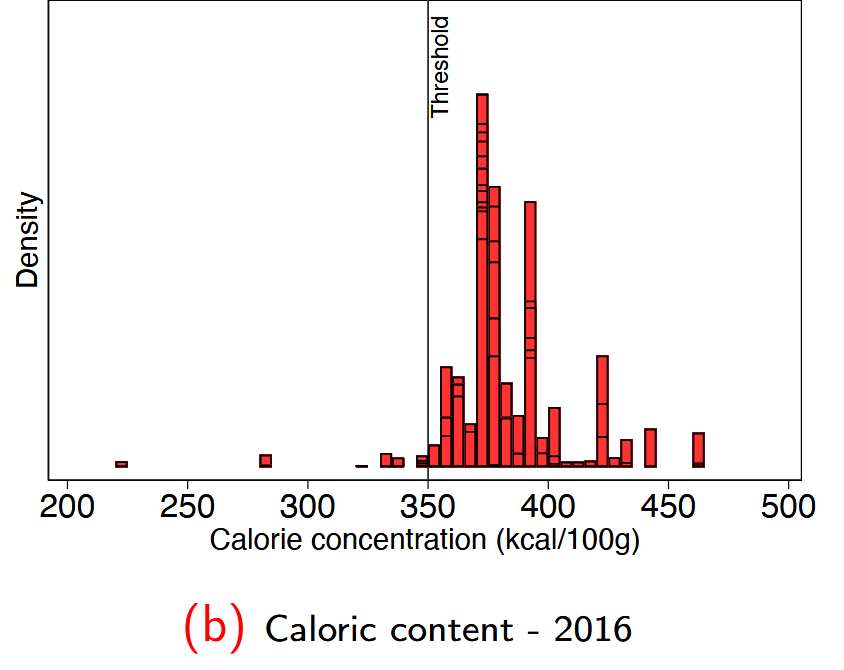
\includegraphics[trim=0cm 2cm 0cm 0cm, clip, width=0.75\linewidth]{bunching_food_labelling_0.png}
    \caption{Before Policy}
    %\label{fig:sub2}
  \end{subfigure}\hfill
  \begin{subfigure}[b]{0.48\textwidth}
    \centering
	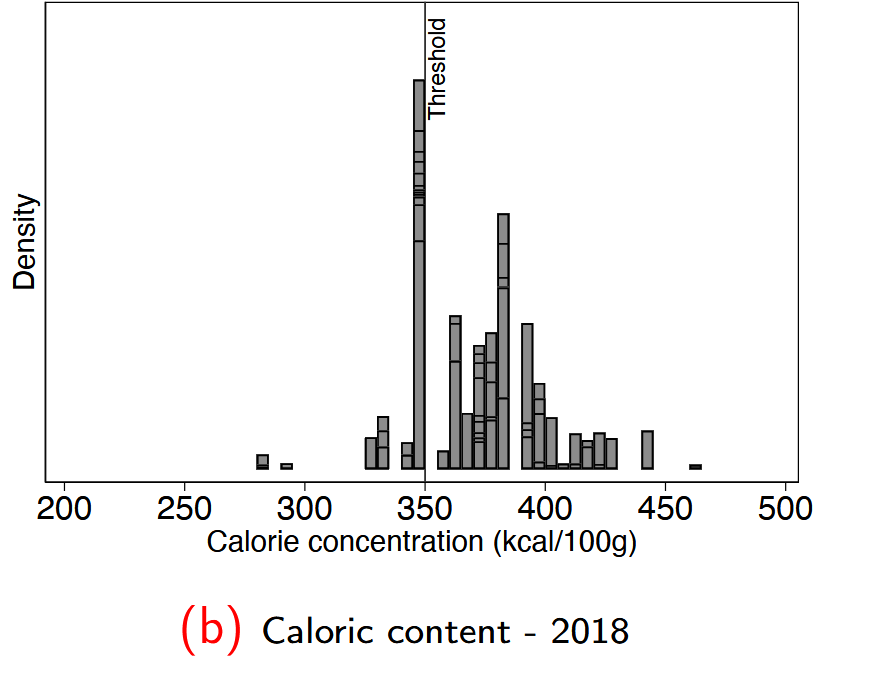
\includegraphics[trim=0cm 2cm 0cm 0cm, clip, width=0.75\linewidth]{bunching_food_labelling_1.png}
    \caption{After Policy}
    %\label{fig:sub2}
  \end{subfigure}
  %\caption{Overall figure caption}
  %\label{fig:two_subfigs}
\end{figure}}
\end{overlayarea}
\end{frame}
			
\begin{frame}{Checking for Manipulation: Bunching}
				
Manipulation of the running variable around the cutoff often generates a big cluster of observations to one side of the cutoff (bunching) and a gap on the other side
	\begin{figure}
					\centering
					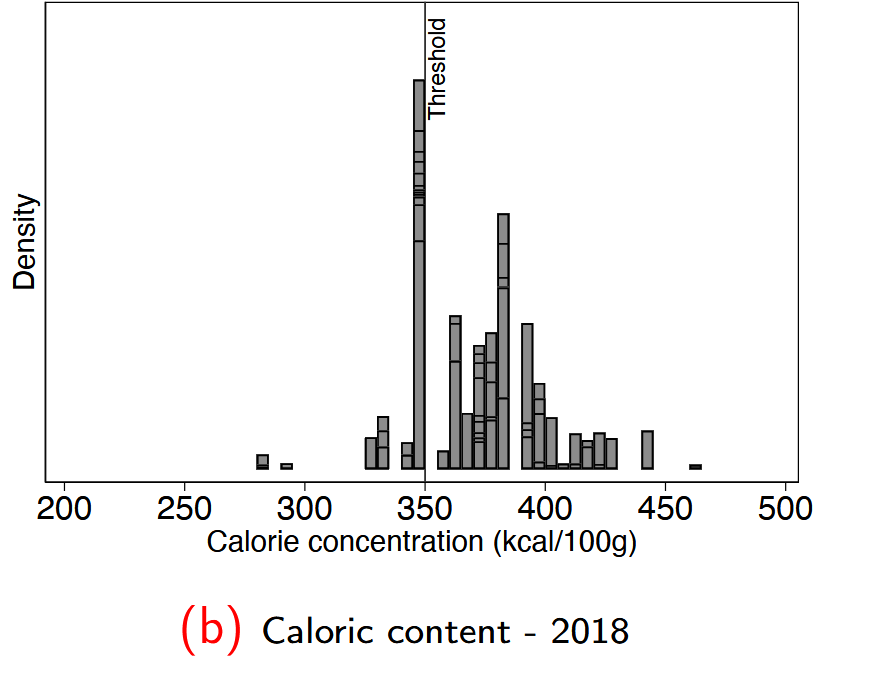
\includegraphics[trim=0cm 2cm 0cm 0cm, clip, width=0.55\linewidth]{bunching_food_labelling_1} \vspace{-0.2cm}
					%\caption{Distribution of Marathon Finishing Times}
	\end{figure}
\end{frame}
			
			
\begin{frame}{Another Issue: Noncompliance}
				
				\textbf{Noncompliance} \\
				The running variable does not fully determine assignment to treatment. At the cutoff, your chance of treatment $increases$ (jumps upward), but not from 0 to 1.
				
				$\rightarrow$ \textbf{Fuzzy RDD} (instead of sharp RDD)
				
				We will not cover the fuzzy RDD in detail, just know that the problem of imperfect determination of allocation to treatment can still be solved.
\end{frame}

\begin{frame}{Coming Up}
				So far, we have discussed the basics of RDD. We will now focus on three practical issues when implementing RDD:
				\begin{enumerate}
					\item Functional form of the running covariate.
					\item Bandwidth choice.
					\item Kernel choice.
				\end{enumerate}
\end{frame}

\section{Functional Form}

\begin{frame}{Fitting the Running Covariate}
	We assumed a \alert{linear} relationship between the running covariate and outcome:
	\begin{align*}
			Deathrate_a = \alert{\alpha + \beta a} + \delta  D_a + u_a 
	\end{align*}
	\pause
	What about trying more flexible specifications? Tradeoff:
		\begin{itemize}
				\item insufficiently flexible: risk of mistaking nonlinearity for treatment effect $\delta$.
				\item overly flexible: reduces precision and runs the risk of overfitting.			
			\pause
				\item essential to visualise the data to choose an appropriate functional form!
		\end{itemize}
	\pause
	The solution: Try different specifications! 
		\begin{enumerate}
			\item linear specification with different slopes above and below the cutoff
			\item Quadratic Polynomial specification
			\item[$\rightarrow$] Treatment coefficient estimates $\hat{\delta}$ across models shouldn't vary too much.
		\end{enumerate}
	\end{frame}
	
\begin{frame}[fragile]{Varying Slopes} 
	Linear functional form, with different slopes \alert{$\beta$}, \alert{$\gamma$} on either side of the cutoff.
	\begin{align*}
		Y = \alpha + \alert{\beta }(a - cutoff) + \alert{\gamma} (a - cutoff) \cdot D_a + \delta  D_a + u_a 
	\end{align*}
	\pause
	\begin{lstlisting}[language=R]
rdd_2slopes <- lm(death_rate_per_100T ~ age_centered*treat, data=df)
coeftest(rdd_2slopes, vcov. = vcovHC(rdd_2slopes, "HC0"))
	\end{lstlisting}
\end{frame}

\begin{frame}{Varying Slopes - Graphical Results}
	\only<1>{
	\begin{figure}
		\centering
		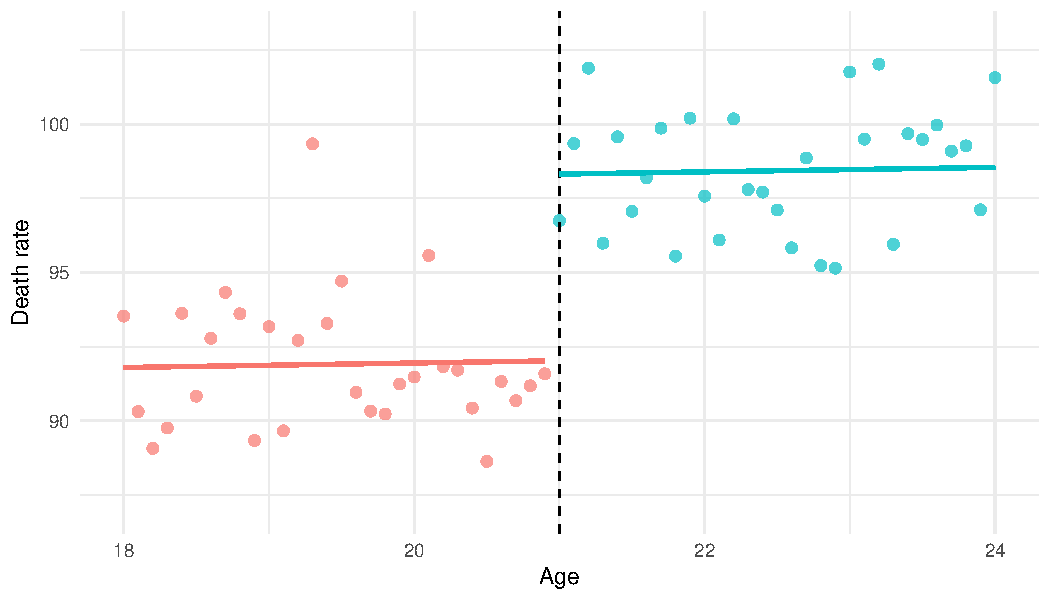
\includegraphics[width =.8\linewidth]{RDD_graph_2.pdf}
	\end{figure}}
	\only<2>{
	\begin{figure}
		\centering
		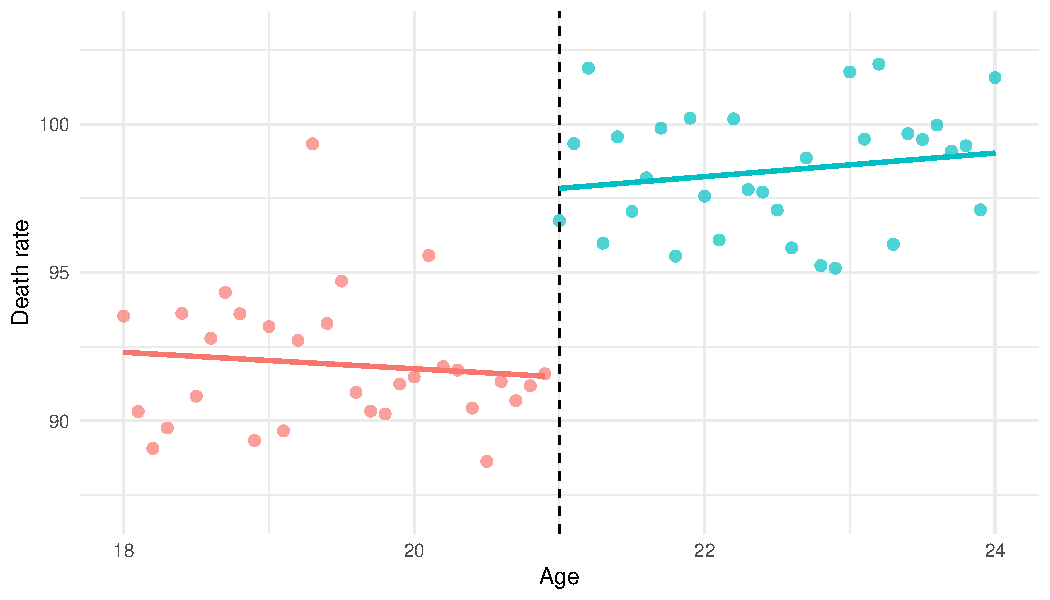
\includegraphics[width =.8\linewidth]{RDD_graph_3.pdf}
	\end{figure}}
\end{frame}

\begin{frame}[fragile]{Quadratic Polynomials} 
	Further improve fit by adding quadratic terms \alert{$\beta_2$}, \alert{$\gamma_2$} below and above cutoff:
	\begin{align*}Y = & \alpha + \beta_1 (a - cutoff) + \alert{\beta_2} (a - cutoff)^2 + \\
					&\gamma_1 (a - cutoff) \cdot D_a + \alert{\gamma_2} (a - cutoff)^2 \cdot D_a  +\delta  D_a + u_a 
	\end{align*} \pause
	\begin{lstlisting}[language=R]
df$age_centered_sq <- (df$age_centered)^2 # new variable

rdd_quadratic <- lm(death_rate_per_100T ~ age_centered*treat + 
					  age_centered_sq*treat, 
					  data=df)

coeftest(rdd_quadratic, vcov. = vcovHC(rdd_quadratic, "HC0"))
	\end{lstlisting}
\end{frame}

\begin{frame}{Quadratic Polynomials - Graphical Results}
	\only<1>{
	\begin{figure}
		\centering
		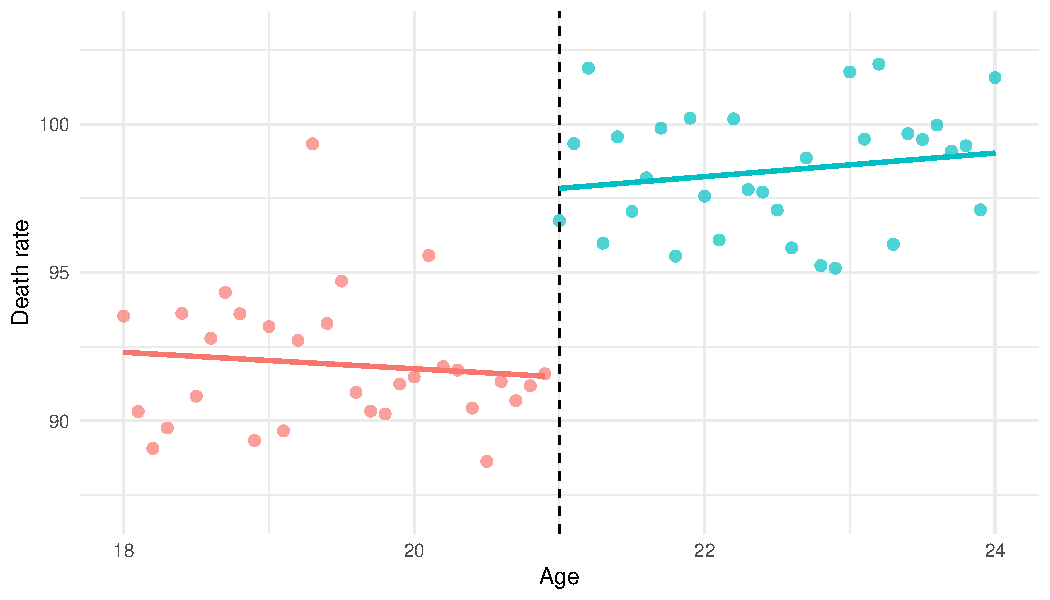
\includegraphics[width =.8\linewidth]{RDD_graph_3.pdf}
	\end{figure}}
	\only<2>{
	\begin{figure}
		\centering
		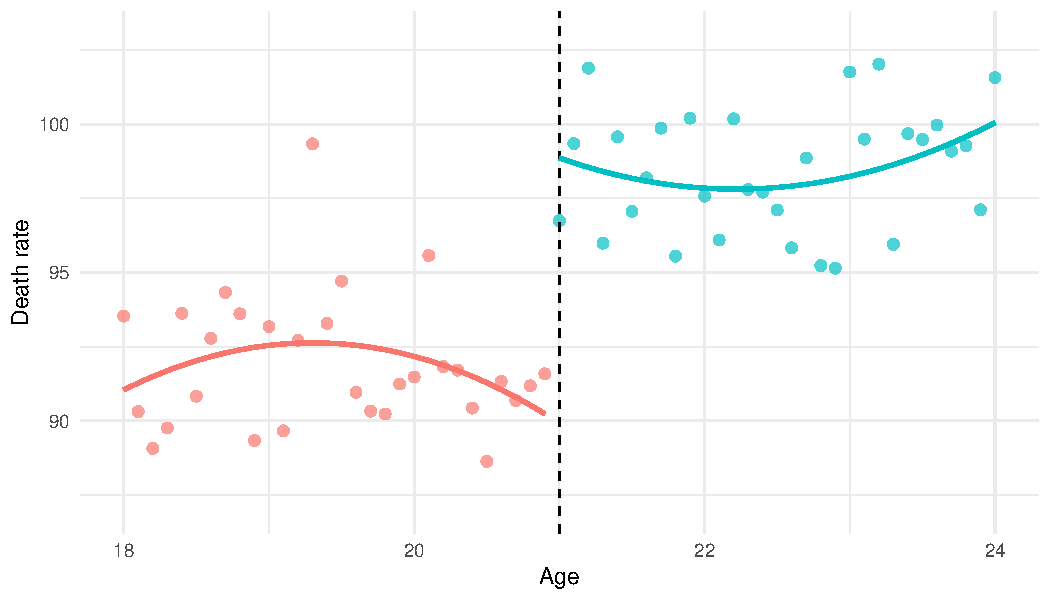
\includegraphics[width =.8\linewidth]{RDD_graph_4.pdf}
	\end{figure}}
\end{frame}

\section{Bandwidth and Kernel}

\begin{frame}{Bandwidth Choice}

\begin{center}
	We want to give \alert{more weight} to observations \alert{closer} to the cutoff level.
\end{center}

\begin{block}{Bandwidth}
				\begin{itemize}
					\item \textbf{Bandwidth} = window around cutoff outside of which you discard observations
					(e.g. only consider individuals aged 19 to 23; or only those aged 20 to 22)
					\item[$\rightarrow$] Narrower bandwidth tradeoff: Assumption credibility v. sample size
				\end{itemize}
\end{block}

\end{frame}
            
\begin{frame}[fragile]{Testing A Narrower Bandwidth}
	New dataset with only observations within 2 years of the cutoff (19-23):
	\begin{lstlisting}[language=R]
df_narrow <- df %>% filter((age_cell>19) & (age_cell<23))
	\end{lstlisting}
	We reproduce the previous specification on the narrower dataset:
	\begin{lstlisting}[language=R]
rdd_quadratic_narrow <- lm(death_rate_per_100T ~ age_centered*treat + 
						age_centered_sq*treat, 
                       	  data=df_narrow)
coeftest(rdd_quadratic_narrow, vcov. = vcovHC(rdd_quadratic_narrow, "HC0"))
	\end{lstlisting}
\end{frame}

\begin{frame}{Narrower Bandwidth - Graphical Results}
	\only<1>{
	\begin{figure}
		\centering
		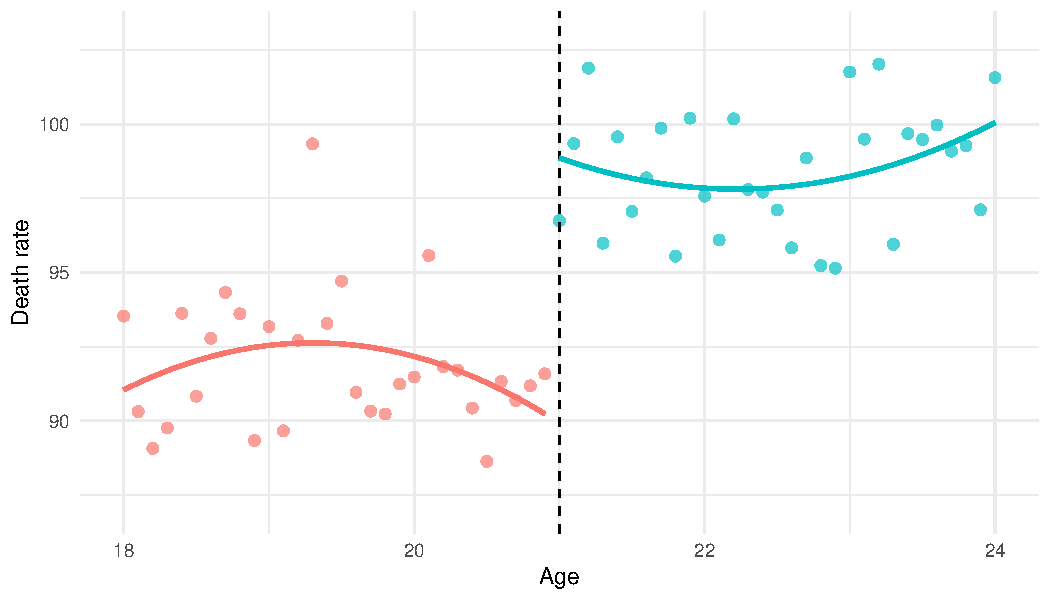
\includegraphics[width =.8\linewidth]{RDD_graph_4.pdf}
	\end{figure}}
	\only<2>{
	\begin{figure}
		\centering
		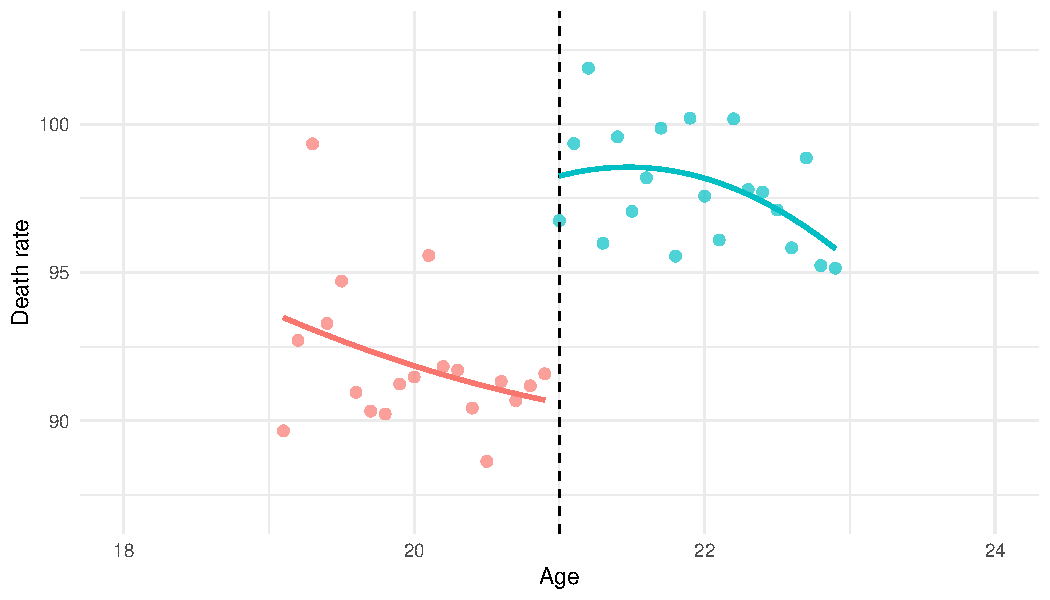
\includegraphics[width =.8\linewidth]{RDD_graph_5.pdf}
	\end{figure}}
\end{frame}

\begin{frame}{Kernel Choice}

\begin{center}
	We want to give \alert{more weight} to observations \alert{closer} to the cutoff level.
\end{center}

\begin{block}{Kernel}
				\begin{itemize}
					\item \textbf{Kernel} = method for assigning importance to values based on their distance to the cutoff
					\item because we care the most about observations right by the cutoff, we typically want to give more distant ones less weight
				\end{itemize}
\end{block}

\end{frame}

\begin{frame}[fragile]{Different Kernels}
\begin{figure}
    \centering
    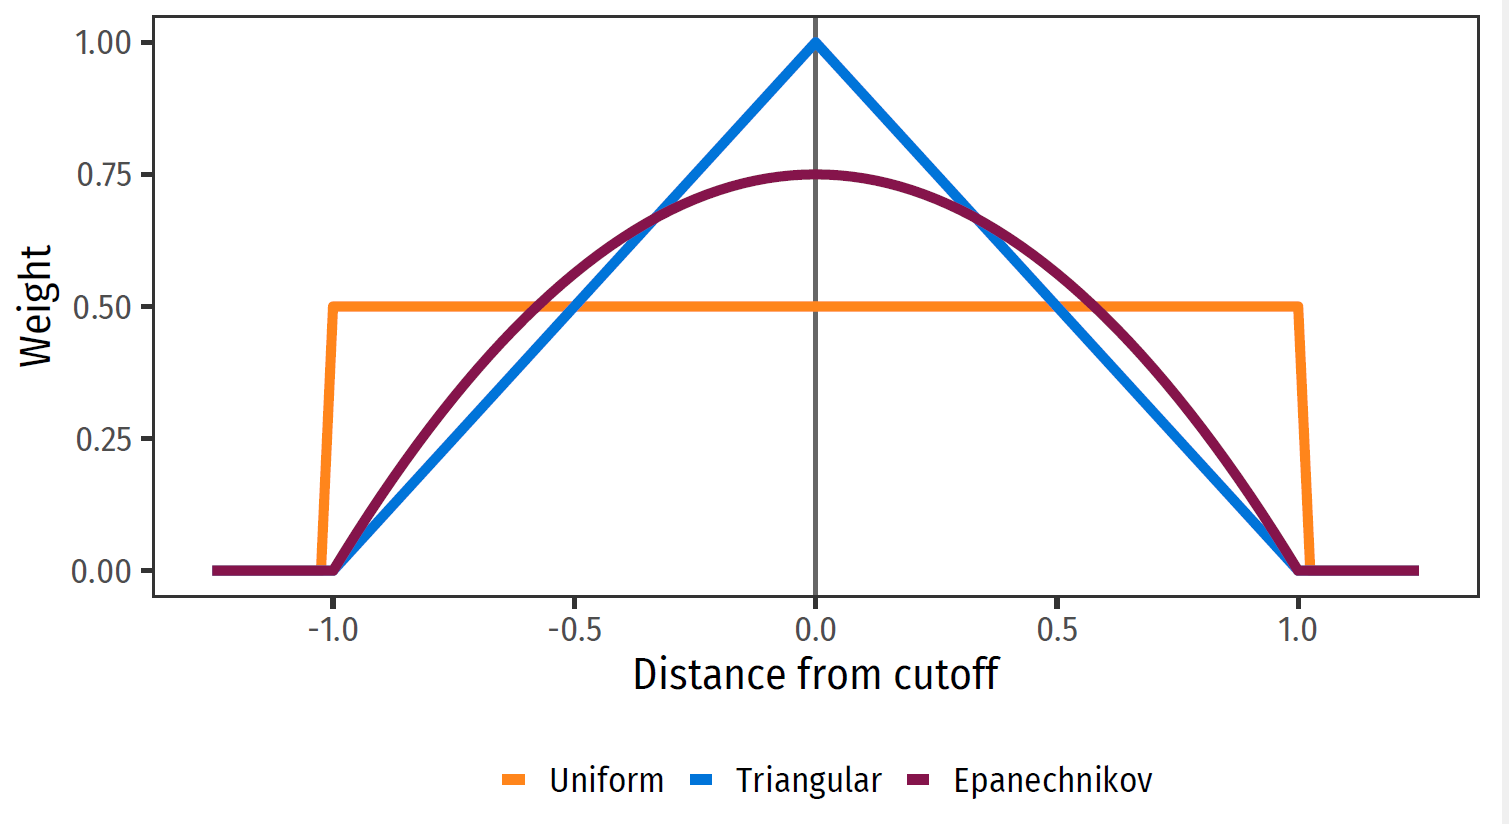
\includegraphics[width=0.85\linewidth]{kernels.png}
     \label{fig:enter-label}\end{figure}
\footnotesize Source: Andrew Heiss 
\end{frame}

\begin{frame}[fragile]{Recap - RDD Implementation}
	
	\begin{itemize}
		\item Recall that implementing RDD requires the research to define:
		\begin{enumerate}
					\item Functional form of the running covariate.
					\item Bandwidth choice
					\item Kernel weighting
		\end{enumerate}
		\item[$\rightarrow$] Different choices can lead to different results! Try them all for robustness.
		%\item The \texttt{rdrobust} R package chooses optimal bandwidth and kernel based on fancy algorithms
	\end{itemize}		
\end{frame}

\end{document}



